%%%%%%%%%%%%%%%%%%%%%%%%%%%%%%%%%%%%%%%%%%%%%%%%%%%%%%%%%%%%%%%%%%%%%%%%%%%%%%%%%%
\begin{frame}[fragile]\frametitle{}
\begin{center}
{\Large Introduction}
\end{center}
\end{frame}

%%%%%%%%%%%%%%%%%%%%%%%%%%%%%%%%%%%%%%%%%%%%%%%%%%%%%%%%%%%%%%%%%%%%%%%%%%%%%%%%%%
\begin{frame}[fragile]\frametitle{Attribution}

Primarily based on:
\begin{itemize}
\item Gartner Hype Cycle Report 2018
\item Gartner Hype Cycle Report 2019
\item Gartner Hype Cycle Report 2020
\end{itemize}
\end{frame}

%%%%%%%%%%%%%%%%%%%%%%%%%%%%%%%%%%%%%%%%%%%%%%%%%%%%%%%%%%%%%%%%%%%%%%%%%%%%%%%%%%
\begin{frame}[fragile]\frametitle{What is a Hype Cycle?}

`` The Gartner Hype Cycle is a device that lays out the path that technologies generally take, from their initial introduction into the market until their eventual maturation into useful components of broader solutions '' - (TBD)


\begin{center}
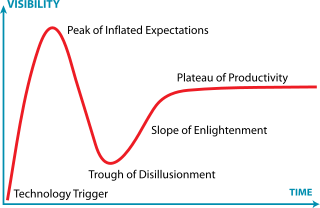
\includegraphics[width=0.4\linewidth,keepaspectratio]{gartner1}
\end{center}

{\tiny (Ref:By Jeremykemp at English Wikipedia, CC BY-SA 3.0, https://commons.wikimedia.org/w/index.php?curid=10547051)}

\end{frame}

%%%%%%%%%%%%%%%%%%%%%%%%%%%%%%%%%%%%%%%%%%%%%%%%%%%%%%%%%%%%%%%%%%%%%%%%%%%%%%%%%%
\begin{frame}[fragile]\frametitle{Phase 1: Technology Trigger}
 \begin{columns}
  \begin{column}{0.55\linewidth}
\begin{itemize}
\item When a new technology is discovered!!
\item Gets mentioned in conferences
\item Enthusiasm
\end{itemize}
  \end{column}%
  \begin{column}{0.45\linewidth}
			\begin{center}
			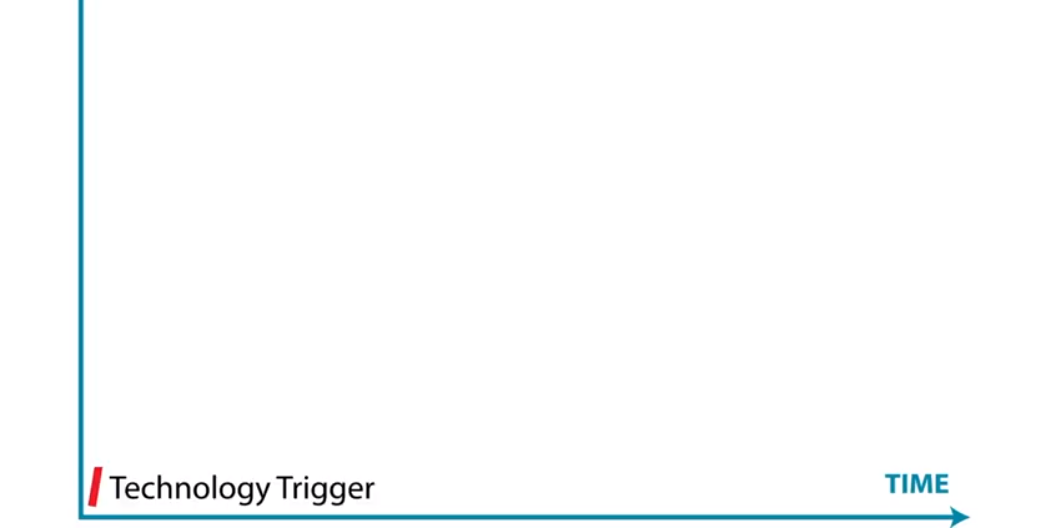
\includegraphics[width=0.9\linewidth,keepaspectratio]{gartner4}
			\end{center}
  \end{column}
 \end{columns}
 
\end{frame}

%%%%%%%%%%%%%%%%%%%%%%%%%%%%%%%%%%%%%%%%%%%%%%%%%%%%%%%%%%%%%%%%%%%%%%%%%%%%%%%%%%
\begin{frame}[fragile]\frametitle{Phase 2: Peak of Inflated Expectations}
 \begin{columns}
  \begin{column}{0.55\linewidth}
\begin{itemize}
\item Gets mentioned even in non-technical forums
\item Seen as solution for ALL problems.
\item E.g. 3D printing my dinner!!
\end{itemize}
  \end{column}%
  \begin{column}{0.45\linewidth}
			\begin{center}
			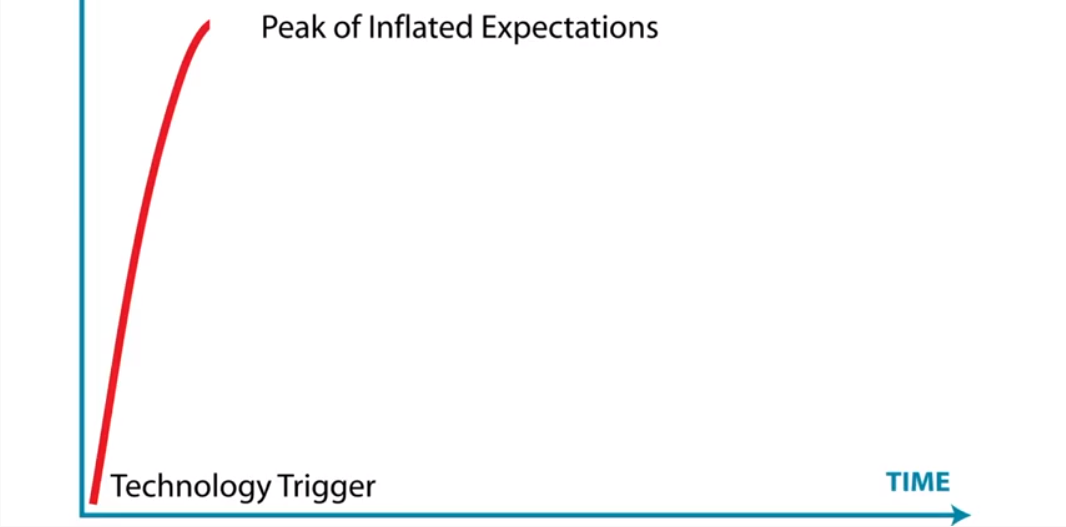
\includegraphics[width=0.9\linewidth,keepaspectratio]{gartner5}
			\end{center}
  \end{column}
 \end{columns}
 
\end{frame}

%%%%%%%%%%%%%%%%%%%%%%%%%%%%%%%%%%%%%%%%%%%%%%%%%%%%%%%%%%%%%%%%%%%%%%%%%%%%%%%%%%
\begin{frame}[fragile]\frametitle{Phase 3: Trough of Disillusionment}
 \begin{columns}
  \begin{column}{0.55\linewidth}
\begin{itemize}
\item Does not live up to ALL expectations
\item Disillusionment
\item Some die here!!
\end{itemize}
  \end{column}%
  \begin{column}{0.45\linewidth}
			\begin{center}
			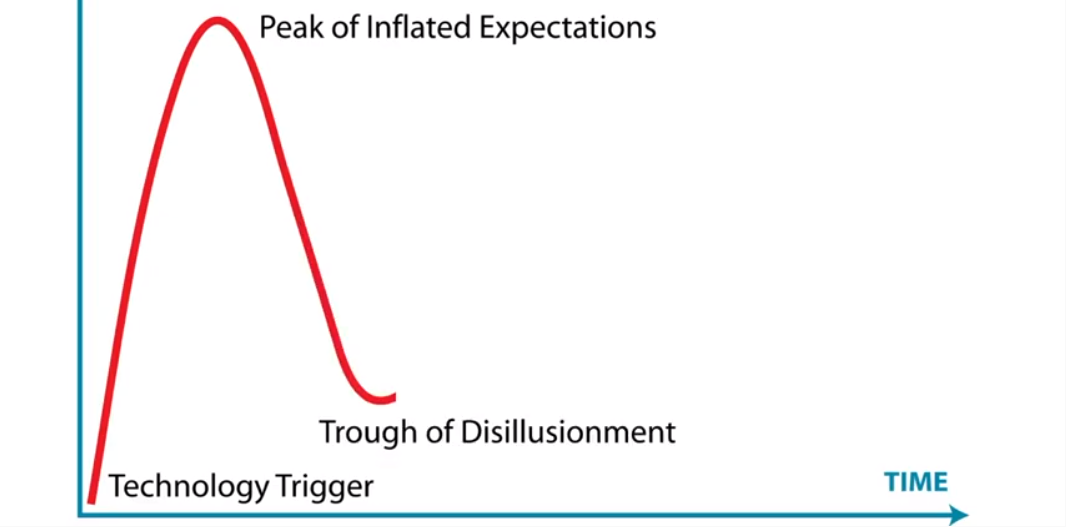
\includegraphics[width=0.9\linewidth,keepaspectratio]{gartner6}
			\end{center}
  \end{column}
 \end{columns}
 
\end{frame}

%%%%%%%%%%%%%%%%%%%%%%%%%%%%%%%%%%%%%%%%%%%%%%%%%%%%%%%%%%%%%%%%%%%%%%%%%%%%%%%%%%
\begin{frame}[fragile]\frametitle{Phase 4: Scope of Enlightenment}
 \begin{columns}
  \begin{column}{0.55\linewidth}
\begin{itemize}
\item Those who survive the trough
\item May not solve ALL the problems but some specific ones.
\item Focused development
\end{itemize}
  \end{column}%
  \begin{column}{0.45\linewidth}
			\begin{center}
			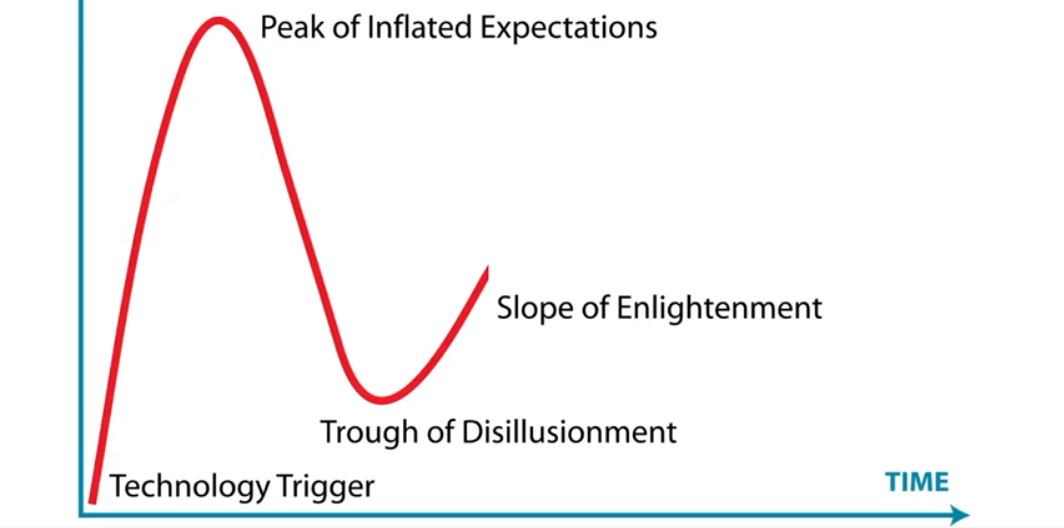
\includegraphics[width=0.9\linewidth,keepaspectratio]{gartner7}
			\end{center}
  \end{column}
 \end{columns}
 
\end{frame}


%%%%%%%%%%%%%%%%%%%%%%%%%%%%%%%%%%%%%%%%%%%%%%%%%%%%%%%%%%%%%%%%%%%%%%%%%%%%%%%%%%
\begin{frame}[fragile]\frametitle{Phase 5: Plateau of Productivity}
 \begin{columns}
  \begin{column}{0.55\linewidth}
\begin{itemize}
\item Good, mature products
\item Survives longer
\end{itemize}
  \end{column}%
  \begin{column}{0.45\linewidth}
			\begin{center}
			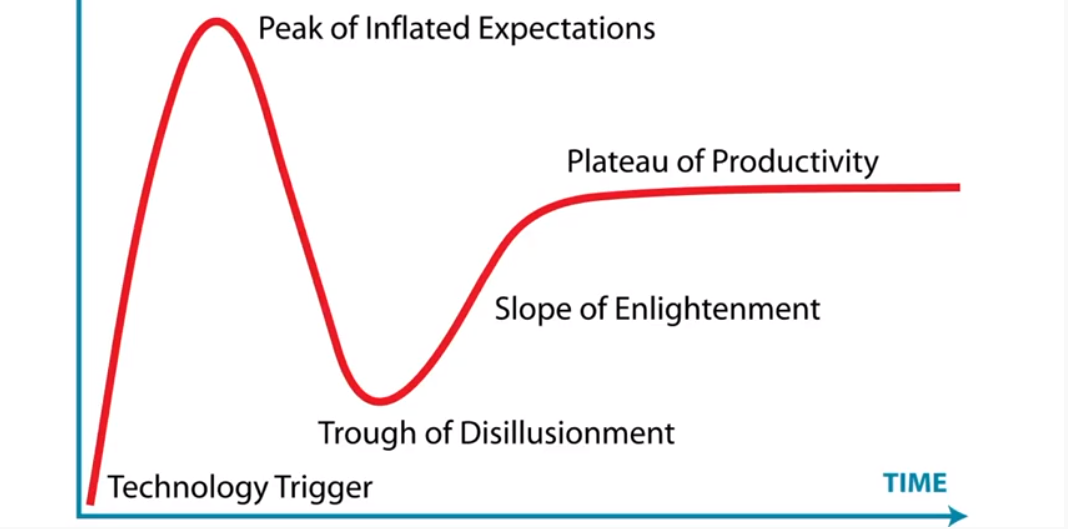
\includegraphics[width=0.9\linewidth,keepaspectratio]{gartner8}
			\end{center}
  \end{column}
 \end{columns}
 
\end{frame}


%%%%%%%%%%%%%%%%%%%%%%%%%%%%%%%%%%%%%%%%%%%%%%%%%%%%%%%%%%%%%%%%%%%%%%%%%%%%%%%%%%
\begin{frame}[fragile]\frametitle{Summary : Phases}

\begin{center}
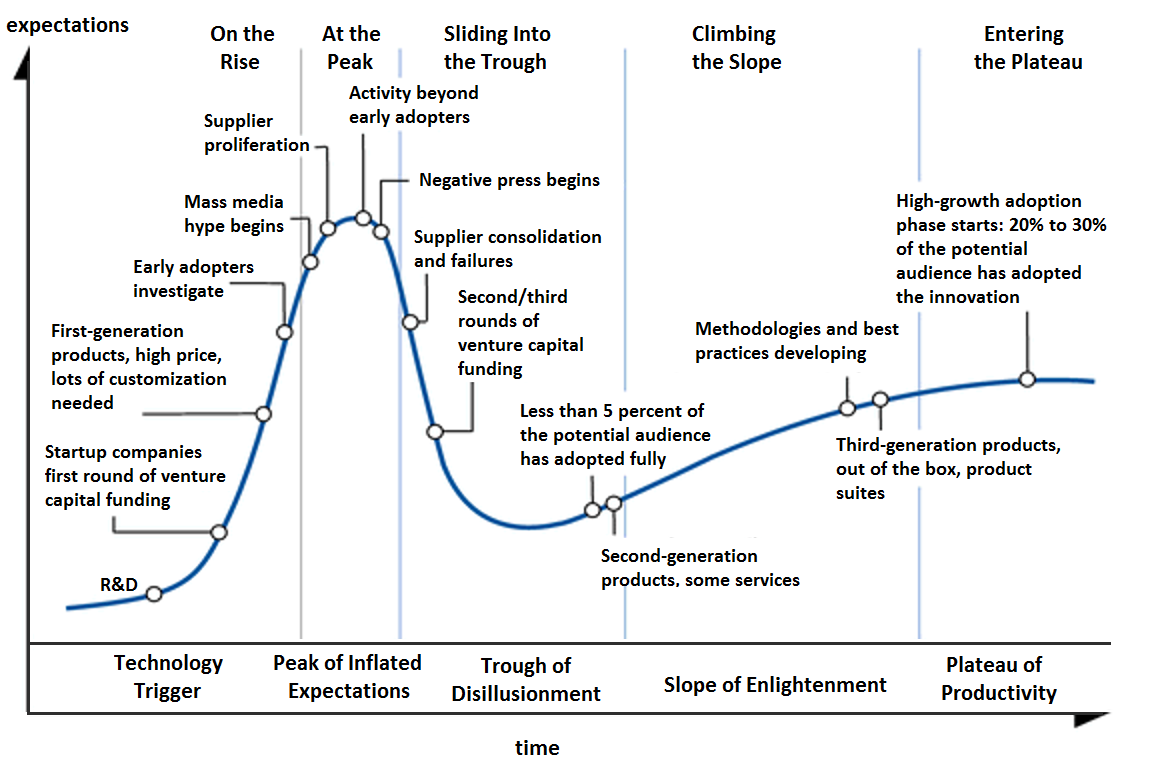
\includegraphics[width=0.8\linewidth,keepaspectratio]{gartner2}
\end{center}

{\tiny (Ref: By NeedCokeNow - Own work, CC BY-SA 3.0, https://commons.wikimedia.org/w/index.php?curid=27546041)}
\end{frame}

%%%%%%%%%%%%%%%%%%%%%%%%%%%%%%%%%%%%%%%%%%%%%%%%%%%%%%%%%%%%%%%%%%%%%%%%%%%%%%%%%%
\begin{frame}[fragile]\frametitle{What it is for?}

``Clients use Hype Cycles to get educated about the promise of an emerging technology within the context of their industry and individual appetite for risk.''

- Gartner 

Hype Cycle distills more than 1,700 unique technologies into a list of must-know technologies and trends.

\end{frame}

%%%%%%%%%%%%%%%%%%%%%%%%%%%%%%%%%%%%%%%%%%%%%%%%%%%%%%%%%%%%%%%%%%%%%%%%%%%%%%%%%%
\begin{frame}[fragile]\frametitle{History of Gartner Hype Cycles?}


\end{frame}

%%%%%%%%%%%%%%%%%%%%%%%%%%%%%%%%%%%%%%%%%%%%%%%%%%%%%%%%%%%%%%%%%%%%%%%%%%%%%%%%%%
\begin{frame}[fragile]\frametitle{Trends in 2018}

\begin{center}
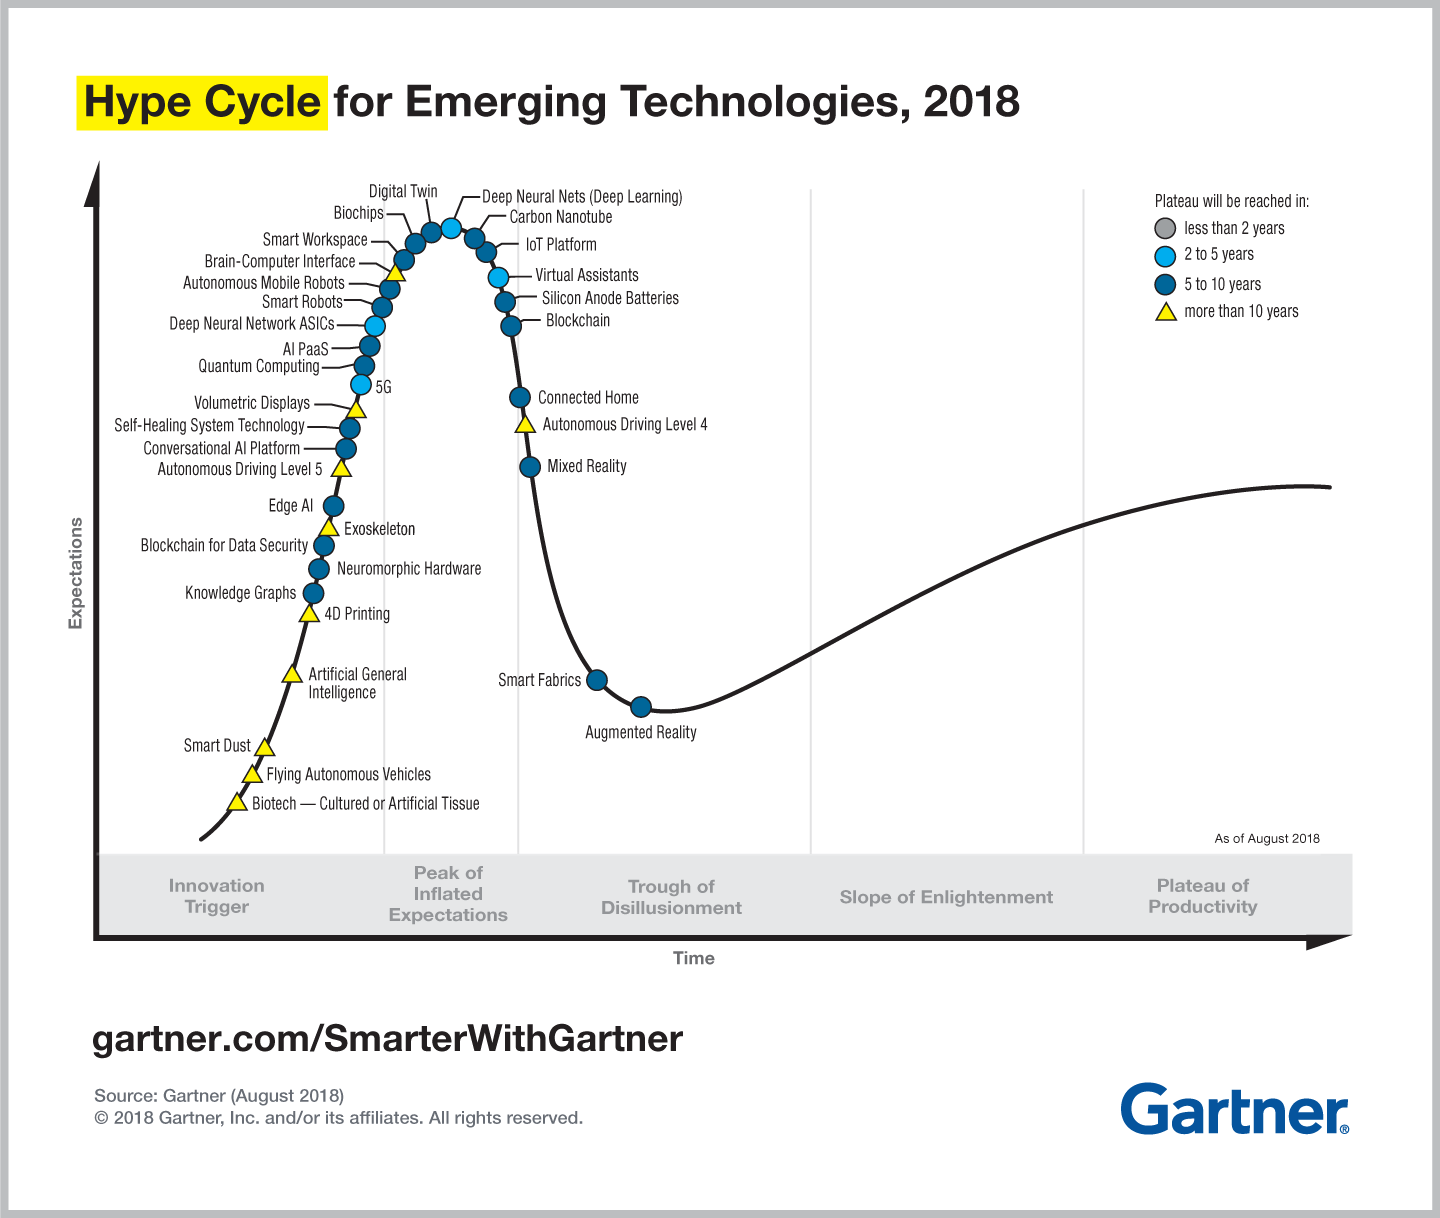
\includegraphics[width=0.7\linewidth,keepaspectratio]{gartner12}
\end{center}


\end{frame}

%%%%%%%%%%%%%%%%%%%%%%%%%%%%%%%%%%%%%%%%%%%%%%%%%%%%%%%%%%%%%%%%%%%%%%%%%%%%%%%%%%
\begin{frame}[fragile]\frametitle{Trends in 2018: Emerging Technologies}
\begin{itemize}
\item Democratized AI, as cloud computing, open source and the "maker" community open AI to the masses.

\item Digitalized ecosystems, as companies shift from compartmentalized infrastructure to platforms that create broader ecosystems to connect humans and tech.

\item Ubiquitous infrastructure, as limitless, always available infrastructure expands business opportunity.

\item Transparently immerse spaces, as technology becomes more human-centric and creates smarter spaces.

\item Do-it-yourself biohacking, as line between what is technology and what is human blurs.

\end{itemize}


{\tiny (Ref:Gartner serves up 2018 Hype Cycle with a heavy side of AI - Alex Hickey)}

\end{frame}

%%%%%%%%%%%%%%%%%%%%%%%%%%%%%%%%%%%%%%%%%%%%%%%%%%%%%%%%%%%%%%%%%%%%%%%%%%%%%%%%%%
\begin{frame}[fragile]\frametitle{Trends in 2019}

\begin{center}
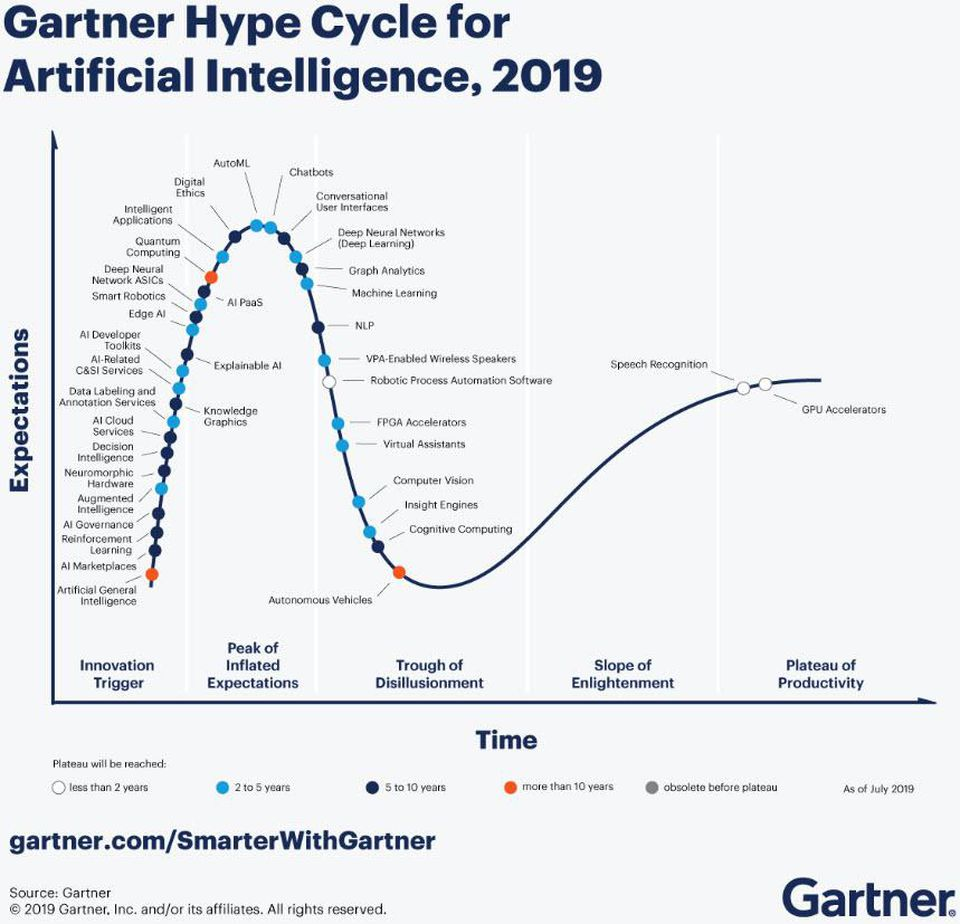
\includegraphics[width=0.7\linewidth,keepaspectratio]{gartner3}
\end{center}

\end{frame}

%%%%%%%%%%%%%%%%%%%%%%%%%%%%%%%%%%%%%%%%%%%%%%%%%%%%%%%%%%%%%%%%%%%%%%%%%%%%%%%%%%
\begin{frame}[fragile]\frametitle{Trends in 2019: Emerging Technologies}
\begin{itemize}
\item Sensing and mobility: light cargo delivery drones, IoT, autonomous driving levels 4 and 5
\item Augmented human: a prosthetic arm that exceeds the strength of a human arm, robotic skin that is as sensitive to touch as human skin
\item Postclassical compute and comms: 5G,  low-earth-orbit (LEO) satellites 
\item Digital ecosystems: Knowledge graphs, synthetic data
\item Advanced AI and analytics: Edge AI, Generative Adversarial Networks

\end{itemize}


{\tiny (Ref: 5 Trends Appear on the Gartner Hype Cycle for Emerging Technologies, 2019 - Kasey Panetta)}

\end{frame}


%%%%%%%%%%%%%%%%%%%%%%%%%%%%%%%%%%%%%%%%%%%%%%%%%%%%%%%%%%%%%%%%%%%%%%%%%%%%%%%%%%
\begin{frame}[fragile]\frametitle{Trends in 2019: AI}

\begin{center}
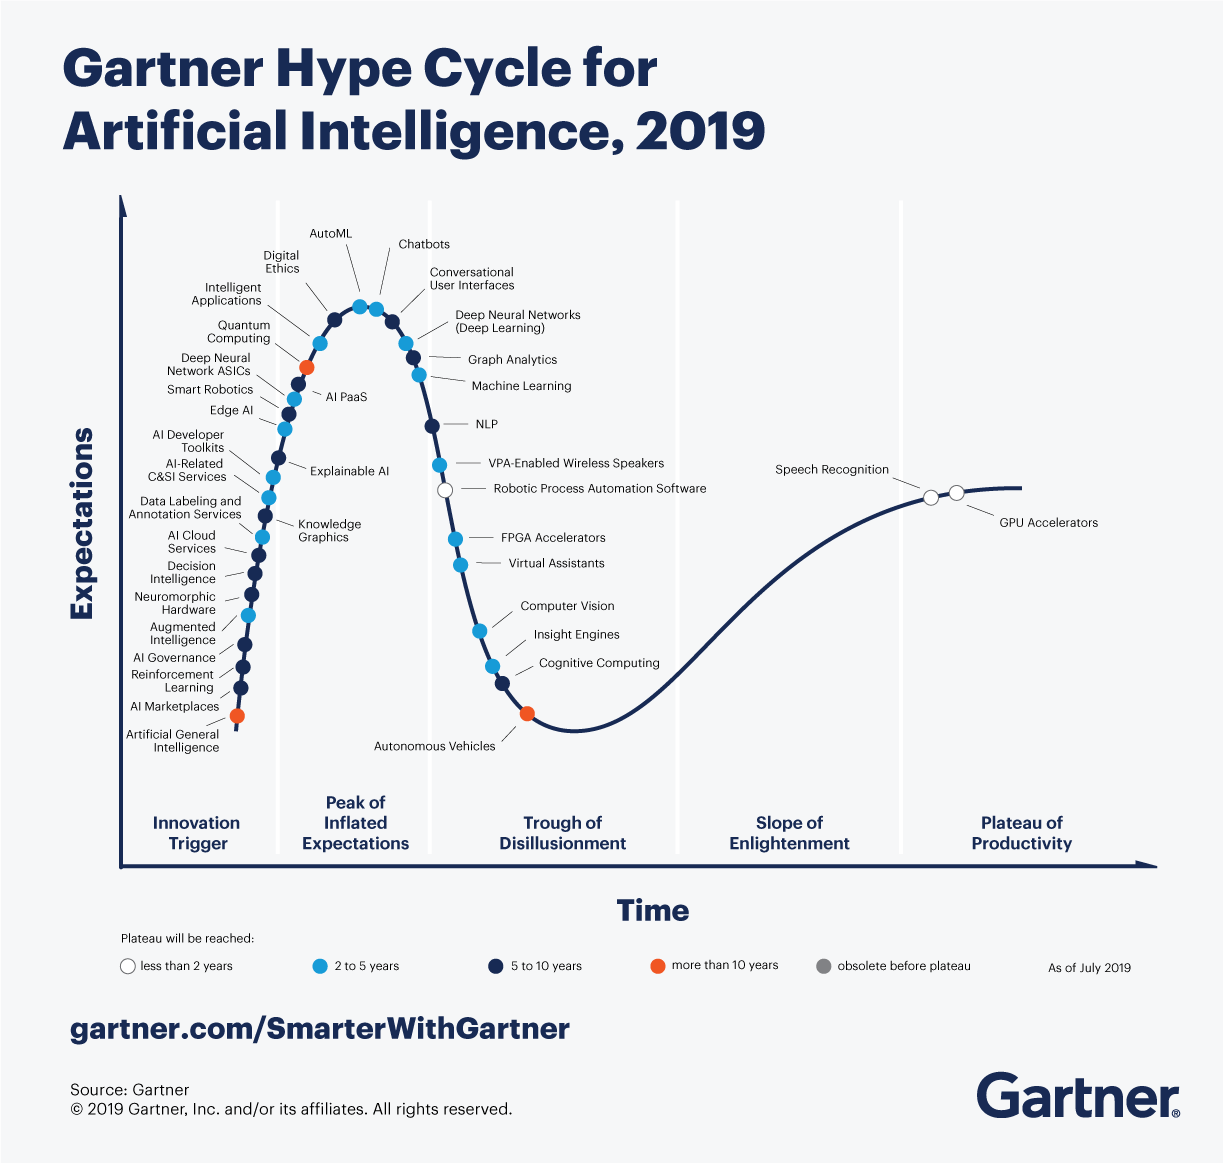
\includegraphics[width=0.7\linewidth,keepaspectratio]{gartner11}
\end{center}

\end{frame}


%%%%%%%%%%%%%%%%%%%%%%%%%%%%%%%%%%%%%%%%%%%%%%%%%%%%%%%%%%%%%%%%%%%%%%%%%%%%%%%%%%
\begin{frame}[fragile]\frametitle{Trends in 2019: AI}
\begin{itemize}
\item Augmented intelligence: to be more efficient with automation, reduce mistakes.
\item Chatbots: The change from “the user learns the interface” to “the chatbot is learning what the user wants” 
\item Machine learning: can solve business problems, due to big data and compute
\item AI governance: creating policies to fight AI-related biases, discrimination and other negative implications of AI
\item Intelligent applications: to support or replace human-based activities via intelligent automation, data-driven insights, and guided recommendations to improve productivity and decision making. 

\end{itemize}


{\tiny (Ref:Top Trends on the Gartner Hype Cycle for Artificial Intelligence, 2019 - 
Laurence Goasduff )}

\end{frame}

%%%%%%%%%%%%%%%%%%%%%%%%%%%%%%%%%%%%%%%%%%%%%%%%%%%%%%%%%%%%%%%%%%%%%%%%%%%%%%%%%%
\begin{frame}[fragile]\frametitle{Trends in 2020}

\begin{center}
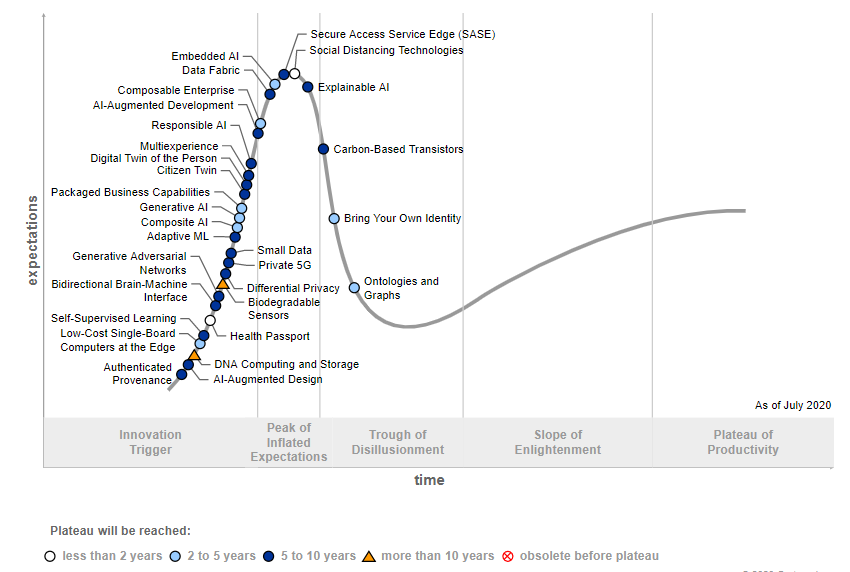
\includegraphics[width=0.7\linewidth,keepaspectratio]{gartner9}
\end{center}


\end{frame}

%%%%%%%%%%%%%%%%%%%%%%%%%%%%%%%%%%%%%%%%%%%%%%%%%%%%%%%%%%%%%%%%%%%%%%%%%%%%%%%%%%
\begin{frame}[fragile]\frametitle{Trends in 2020: Emerging Technologies}

Unique trends:

\begin{itemize}
\item Composite architectures: plug-and-play like Lego blocks, packaged business capabilities built on a flexible data fabric, to respond to rapidly changing business needs.
\item Algorithmic trust: to shift from trusting central authorities to trusting algorithms, Block-chain
\item Beyond silicon: Use synthetic DNA in place of silicon or quantum architectures to perform computation or store data. (still rudimentary)
\item Formative AI: adaptive ML, generative AI to create new novel content (images, video etc.) or alter existing content
\item Digital me: digital versions of ourselves, health digital twins, authentication, access and payment.
\end{itemize}


{\tiny (Ref: 5 Trends Drive the Gartner Hype Cycle for Emerging Technologies, 2020 - Laurence Goasduff )}

\end{frame}

%%%%%%%%%%%%%%%%%%%%%%%%%%%%%%%%%%%%%%%%%%%%%%%%%%%%%%%%%%%%%%%%%%%%%%%%%%%%%%%%%%
\begin{frame}[fragile]\frametitle{Trends in 2020: AI}

\begin{center}
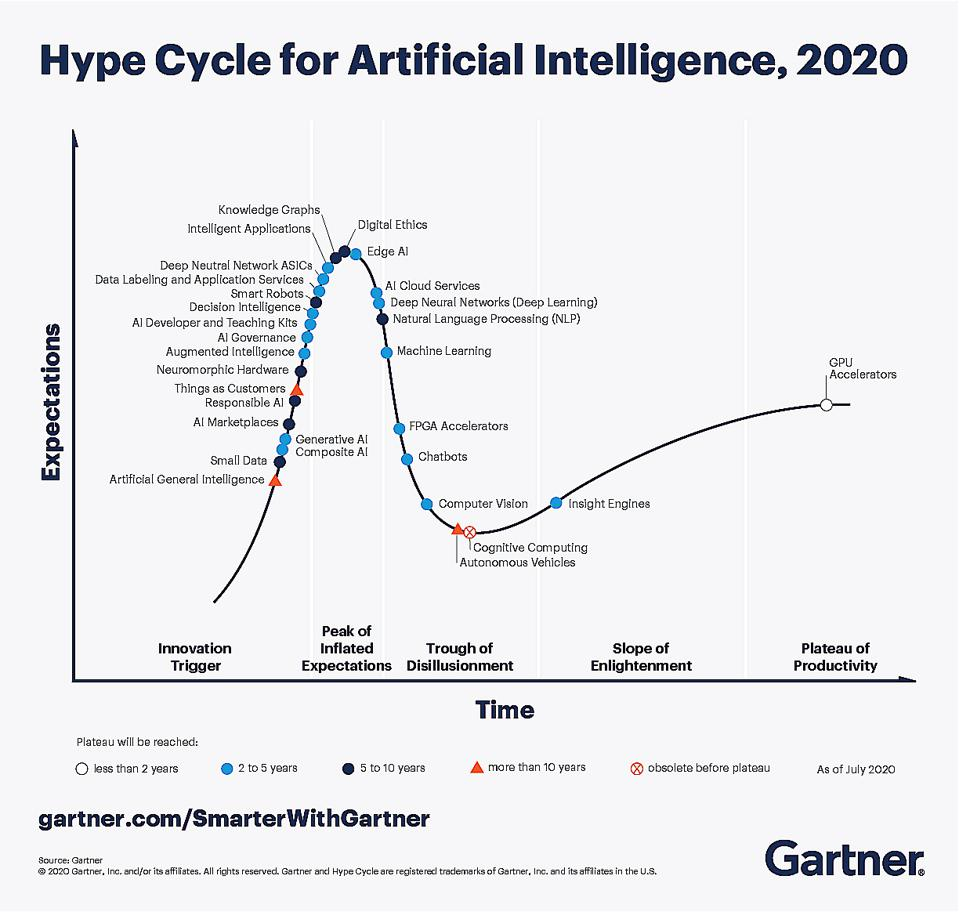
\includegraphics[width=0.7\linewidth,keepaspectratio]{gartner10}
\end{center}

{\tiny (Ref:2 Megatrends Dominate the Gartner Hype Cycle for Artificial Intelligence, 2020 - Laurence Goasduff )}

\end{frame}

%%%%%%%%%%%%%%%%%%%%%%%%%%%%%%%%%%%%%%%%%%%%%%%%%%%%%%%%%%%%%%%%%%%%%%%%%%%%%%%%%%
\begin{frame}[fragile]\frametitle{Trends in 2020: AI}

\begin{itemize}
\item In spite of COVID, nearly half of AI investments intact. About a third are planning to increase. 16\% suspended and 7\% decreased the investments.
\item AI is starting to deliver
\item Five new entrants — small data, generative AI, composite AI, responsible AI and things as customers
\item Two mega trends: Democratization, Industrialization
\end{itemize}


{\tiny (Ref:2 Megatrends Dominate the Gartner Hype Cycle for Artificial Intelligence, 2020 - Laurence Goasduff )}

\end{frame}

%%%%%%%%%%%%%%%%%%%%%%%%%%%%%%%%%%%%%%%%%%%%%%%%%%%%%%%%%%%%%%%%%%%%%%%%%%%%%%%%%%
\begin{frame}[fragile]\frametitle{Trends in 2020: Democratization of Artificial Intelligence}

\begin{itemize}
\item `` Gartner foresees developers being the major force in AI''
\item Along with data scientists and data engineers, developers would be key.
\item Engineering complements data science to deliver AI at scale
\end{itemize}


{\tiny (Ref:2 Megatrends Dominate the Gartner Hype Cycle for Artificial Intelligence, 2020 - Laurence Goasduff )}

\end{frame}

%%%%%%%%%%%%%%%%%%%%%%%%%%%%%%%%%%%%%%%%%%%%%%%%%%%%%%%%%%%%%%%%%%%%%%%%%%%%%%%%%%
\begin{frame}[fragile]\frametitle{Trends in 2020: Industrialization of AI platforms
}

\begin{itemize}
\item `` Responsible AI and AI governance also become a priority for AI on an industrial scale''
\item Enables the reusability, scalability and safety of AI, which accelerates its adoption and growth.
\end{itemize}


{\tiny (Ref:2 Megatrends Dominate the Gartner Hype Cycle for Artificial Intelligence, 2020 - Laurence Goasduff )}

\end{frame}

%%%%%%%%%%%%%%%%%%%%%%%%%%%%%%%%%%%%%%%%%%%%%%%%%%%%%%%%%%%%%%%%%%%%%%%%%%%%%%%%%%
\begin{frame}[fragile]\frametitle{Trends in 2020: AI}

\begin{itemize}
\item Chatbots: 100\% increase in adoption rates in 2-5 years
\item GPU Accelerators are the nearest-term technology to mainstream adoption
\item AI-based minimum viable products replacing pilot projects 
\item To focus on narrow AI than the General AI, as it is not commercially viable.
\item Small data, Generative AI  enter Hype Cycle.
\item Responsible AI: Concentrating on the ethical and social aspects of AI
\item Things as Customers: a smart device or machine or that obtains goods or services in exchange for payment
\end{itemize}


{\tiny (Ref:What’s New In Gartner’s Hype Cycle For AI, 2020 - 
Louis Columbus )}

\end{frame}

%%%%%%%%%%%%%%%%%%%%%%%%%%%%%%%%%%%%%%%%%%%%%%%%%%%%%%%%%%%%%%%%%%%%%%%%%%%%%%%%%%
\begin{frame}[fragile]\frametitle{Trends in 2020: Embedded AI}
\begin{itemize}
\item Stage: Peak of inflated expectations
\item Time required to plateau: 2 to 5 years
\item Supercomputers in the pockets, Edge computing systems
\item Era of IoT, 5G and portable medical devices
\item Applications for manufacturing, retail, smart cities, and more
\end{itemize}


{\tiny (Ref:AI Technologies That Featured In Latest Gartner Hype Cycle - 
Ram Sagar )}

\end{frame}

%%%%%%%%%%%%%%%%%%%%%%%%%%%%%%%%%%%%%%%%%%%%%%%%%%%%%%%%%%%%%%%%%%%%%%%%%%%%%%%%%%
\begin{frame}[fragile]\frametitle{Trends in 2020: Generative AI}
\begin{itemize}
\item Stage: Innovation Trigger
\item Time required to plateau: 2 to 5 years
\item Paint auction-worthy art, generate songs and even create faces of people who never existed. 
\item Disadvantage: Malicious online players can now generate disinformation in the form of images and videos that can fool many. 
\end{itemize}


{\tiny (Ref:AI Technologies That Featured In Latest Gartner Hype Cycle - 
Ram Sagar )}

\end{frame}

%%%%%%%%%%%%%%%%%%%%%%%%%%%%%%%%%%%%%%%%%%%%%%%%%%%%%%%%%%%%%%%%%%%%%%%%%%%%%%%%%%
\begin{frame}[fragile]\frametitle{Trends in 2020: Responsible And Explainable AI}
\begin{itemize}
\item Stage: Innovation Trigger \& Peak of inflated expectations resp.
\item Time required to plateau: 5 to 10 years
\item Machine learning algorithms are infamous for their black-box nature
\item Growing demand for explain-ability
\item Medical diagnosis or credit card risk estimation
\end{itemize}


{\tiny (Ref:AI Technologies That Featured In Latest Gartner Hype Cycle - 
Ram Sagar )}

\end{frame}

%%%%%%%%%%%%%%%%%%%%%%%%%%%%%%%%%%%%%%%%%%%%%%%%%%%%%%%%%%%%%%%%%%%%%%%%%%%%%%%%%%
\begin{frame}[fragile]\frametitle{Trends in 2020: Self Supervised Learning}
\begin{itemize}
\item Stage: Innovation Trigger
\item Time required to plateau: 5 to 10 years
\item Availability of pre-trained models are almost negligible due to less data, needing more accurate results
\end{itemize}


{\tiny (Ref:AI Technologies That Featured In Latest Gartner Hype Cycle - 
Ram Sagar )}

\end{frame}


%%%%%%%%%%%%%%%%%%%%%%%%%%%%%%%%%%%%%%%%%%%%%%%%%%%%%%%%%%%%%%%%%%%%%%%%%%%%%%%%%%
\begin{frame}[fragile]\frametitle{Trends in 2020: AI Augmented Development}
\begin{itemize}
\item Stage: Peak of inflated expectations
\item Time required to plateau: 5 to 10 years
\item AI assisting organizations in design, development and deployment of their software products
\item To take care of the mundane debugging tasks through automation.
\end{itemize}


{\tiny (Ref:AI Technologies That Featured In Latest Gartner Hype Cycle - 
Ram Sagar )}

\end{frame}



%%%%%%%%%%%%%%%%%%%%%%%%%%%%%%%%%%%%%%%%%%%%%%%%%%%%%%%%%%%%%%%%%%%%%%%%%%%%%%%%%%
\begin{frame}[fragile]\frametitle{Transitions}

\begin{itemize}
\item Thirteen technologies have either been removed, re-classified, or moved to other Hype Cycles compared to last year.
\item Robotic process automation software is now removed 
\item Graph analytics and Reinforcement Learning to the Hype Cycle for Data Science and Machine Learning, 2020
\end{itemize}



\end{frame}



%%%%%%%%%%%%%%%%%%%%%%%%%%%%%%%%%%%%%%%%%%%%%%%%%%%%%%%%%%%%%%%%%%%%%%%%%%%%%%%%%%
\begin{frame}[fragile]\frametitle{Criticism By Patrick Crouch}


\begin{itemize}
\item Personally, couldn’t find a single example of tech-oriented company using the Hype Cycle to determine spending or strategy.
\item So who’s using it? Answer: Marketers.
\item Most technological advances come from the combination or misuse of a variety of technologies, not from one technology being researched
\item The Gartner Hype Cycle is more of a scapegoat for failing/unrealized technical promise than a useful tool

\end{itemize}

{\tiny (Ref: The Gartner Hype Cycle - Does the Gartner Hype Cycle Invalidate Itself? - By: Patrick Crouch)}

\end{frame}


%%%%%%%%%%%%%%%%%%%%%%%%%%%%%%%%%%%%%%%%%%%%%%%%%%%%%%%%%%%%%%%%%%%%%%%%%%%%%%%%%%
\begin{frame}[fragile]\frametitle{}
\begin{center}
{\Large Conclusion}
\end{center}
\end{frame}

%%%%%%%%%%%%%%%%%%%%%%%%%%%%%%%%%%%%%%%%%%%%%%%%%%%%%%%%%%%%%%%%%%%%%%%%%%%%%%%%%%
\begin{frame}[fragile]\frametitle{What Next?}


\begin{itemize}
\item Build Solid foundation in Data Sciences, Machine Learning, Deep Learning, etc.
\item Don't ignore seemingly mundane, Data Engineering and Results Interpretation.
\item Build specific domain expertise and projects therein.
\item Github, Kaggle, Meetups \ldots
\end{itemize}

\end{frame}


%%%%%%%%%%%%%%%%%%%%%%%%%%%%%%%%%%%%%%%%%%%%%%%%%%%%%%%%%%%%%%%%%%%%%%%%%%%%%%%%%%
\begin{frame}[fragile]\frametitle{Additional References}


\begin{itemize}
\item What's New In Gartner's Hype Cycle For AI, 2019 - Louis Columbus
\item Gartner Hype Cycle - J Scott Christianson
\end{itemize}

\end{frame}

% %%%%%%%%%%%%%%%%%%%%%%%%%%%%%%%%%%%%%%%%%%%%%%%%%%%%%%%%%%%%%%%%%%%%%%%%%%%%%%%%%%
% \begin{frame}[fragile]{Evolution of CAD Technology}
% \begin{center}
% \includegraphics[width=0.9\linewidth,keepaspectratio]{geomod1}
% \end{center}
% \end{frame}

% %%%%%%%%%%%%%%%%%%%%%%%%%%%%%%%%%%%%%%%%%%%%%%%%%%%%%%%%%%%%%%%%%%%%%%%%%%%%%%%%%%
% \begin{frame}[fragile]{Manual drafting}
 % \begin{columns}
  % \begin{column}{0.55\linewidth}
% \begin{itemize}
% \item 2D representations used to represent 3D objects
% \begin{itemize}
% \item multi-view drawings
% \item pictorials
% \end{itemize}
% \item Standards and conventions developed so that 3D object could be built from drawings
% \item Drawings created manually or using 2D CAD
% \item Difficult to visualize, error-prone, time-consuming
% \end{itemize}
  % \end{column}%
  % \begin{column}{0.45\linewidth}
			% \begin{center}
			% \includegraphics[width=0.9\linewidth,keepaspectratio]{geomod2}
			% \end{center}
  % \end{column}
 % \end{columns}
% \end{frame}

